\documentclass[letterpaper,12pt]{scrartcl}
\usepackage[utf8]{inputenc}
\usepackage[english]{babel}

%==============================================================================
% CUSTOM STYLE
%==============================================================================
\usepackage{simple-report-template}

%==============================================================================
% BIBLIOGRAPHY
%==============================================================================
\usepackage{csquotes}
\usepackage[backend=biber,style=authoryear,maxcitenames=2]{biblatex}
\addbibresource{references.bib}

% Make \cite behave like \textcite (Author (Year) format)
\let\cite\textcite

%==============================================================================
% HYPERLINKS
%==============================================================================
\usepackage{hyperref}

%==============================================================================
% HEADER SETUP
%==============================================================================
\setupheader{Northvale Institute of Technology}{Department of Engineering}{Fall Semester 2025}{Thesis Workshop - ENG-231}

%==============================================================================
% DOCUMENT
%==============================================================================
\begin{document}

%==============================================================================
% TITLE PAGE
%==============================================================================
\maketitlepage
{NORTHVALE \ INSTITUTE \ OF \ TECHNOLOGY}
{Department of Engineering}
{Analysis of Structural Performance in Modern Architecture}
{Master Thesis Progress Report}
{\authorinfo{Prof. Michael Anderson}{Emily Rodriguez}{Sunday 9th November 2025}}

%==============================================================================
% TABLE OF CONTENTS
%==============================================================================
\thispagestyle{empty}
\tableofcontents
\newpage

%==============================================================================
% CONTENT
%==============================================================================

\section{Introduction}

Lorem ipsum dolor sit amet, consectetur adipiscing elit. Sed do eiusmod tempor incididunt ut labore et dolore magna aliqua. Ut enim ad minim veniam, quis nostrud exercitation ullamco laboris nisi ut aliquip ex ea commodo consequat \textcite{smith2020}.

Duis aute irure dolor in reprehenderit in voluptate velit esse cillum dolore eu fugiat nulla pariatur. Excepteur sint occaecat cupidatat non proident, sunt in culpa qui officia deserunt mollit anim id est laborum.

\subsection{Background}

Sed ut perspiciatis unde omnis iste natus error sit voluptatem accusantium doloremque laudantium, totam rem aperiam, eaque ipsa quae ab illo inventore veritatis et quasi architecto beatae vitae dicta sunt explicabo \parencite{johnson2019}.

Nemo enim ipsam voluptatem quia voluptas sit aspernatur aut odit aut fugit, sed quia consequuntur magni dolores eos qui ratione voluptatem sequi nesciunt.

\subsection{Objectives}

At vero eos et accusamus et iusto odio dignissimos ducimus qui blanditiis praesentium voluptatum deleniti atque corrupti quos dolores et quas molestias excepturi sint occaecati cupiditate non provident.

\begin{enumerate}
    \item Investigate structural performance under various load conditions
    \item Develop computational models for stress analysis
    \item Validate results against experimental data
    \item Propose design optimization strategies
\end{enumerate}

\section{Methodology}

Temporibus autem quibusdam et aut officiis debitis aut rerum necessitatibus saepe eveniet ut et voluptates repudiandae sint et molestiae non recusandae.

\subsection{Phase 1: Data Collection}

\begin{itemize}
    \item Survey of existing structures
    \item Material property testing
    \item Load measurement and monitoring
    \item Environmental condition assessment
\end{itemize}

Itaque earum rerum hic tenetur a sapiente delectus, ut aut reiciendis voluptatibus maiores alias consequatur aut perferendis doloribus asperiores repellat.

\subsection{Phase 2: Analysis}

Nam libero tempore, cum soluta nobis est eligendi optio cumque nihil impedit quo minus id quod maxime placeat facere possimus, omnis voluptas assumenda est, omnis dolor repellendus.

\begin{equation}
    \sigma = \frac{F}{A}
    \label{eq:stress}
\end{equation}

The stress $\sigma$ is calculated according to equation \ref{eq:stress}, where $F$ represents the applied force and $A$ the cross-sectional area.

\subsection{Phase 3: Validation}

Temporibus autem quibusdam et aut officiis debitis aut rerum necessitatibus saepe eveniet ut et voluptates repudiandae sint et molestiae non recusandae.

\section{Results}

On the other hand, we denounce with righteous indignation and dislike men who are so beguiled and demoralized by the charms of pleasure of the moment, so blinded by desire, that they cannot foresee the pain and trouble.

\subsection{Structural Analysis}

These cases are perfectly simple and easy to distinguish. In a free hour, when our power of choice is untrammelled and when nothing prevents our being able to do what we like best, every pleasure is to be welcomed.

\begin{figure}[h]
\centering
% Example figure using TikZ
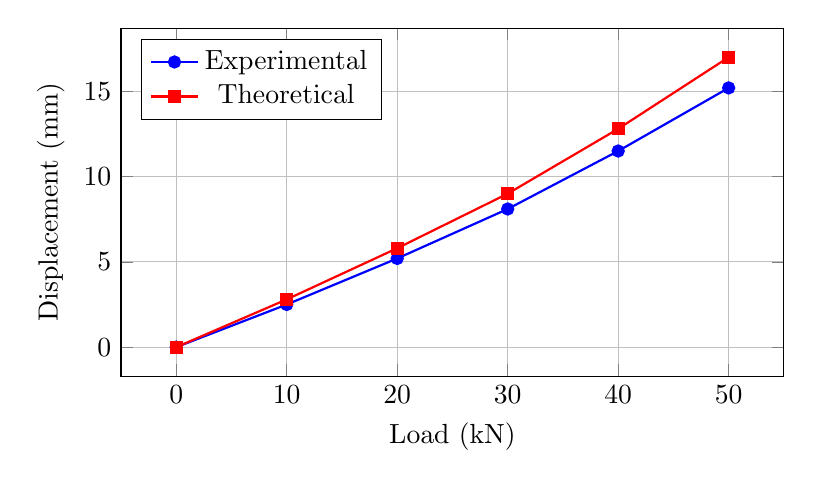
\begin{tikzpicture}
    \begin{axis}[
        width=10cm,
        height=6cm,
        xlabel={Load (kN)},
        ylabel={Displacement (mm)},
        grid=major,
        legend pos=north west,
    ]
    \addplot[blue, thick, mark=*] coordinates {
        (0,0) (10,2.5) (20,5.2) (30,8.1) (40,11.5) (50,15.2)
    };
    \addplot[red, thick, mark=square*] coordinates {
        (0,0) (10,2.8) (20,5.8) (30,9.0) (40,12.8) (50,17.0)
    };
    \legend{Experimental, Theoretical}
    \end{axis}
\end{tikzpicture}

\caption{Load-displacement relationship comparing experimental and theoretical results.}
\label{fig:load-displacement}
\end{figure}

As shown in Figure \ref{fig:load-displacement}, the experimental results closely follow the theoretical predictions, with minor deviations observed at higher load levels.

\subsection{Tables Example}

\begin{table}[h]
\caption{Comparison of structural materials and their properties.}
\label{tab:materials}
\centering
\begin{tabular}{lcccc}
\hline
\textbf{Material} & \textbf{Strength (MPa)} & \textbf{Density (kg/m³)} & \textbf{Cost (USD/kg)} & \textbf{Rating} \\
\hline
Steel A36 & 250 & 7850 & 0.85 & 4.2 \\
Aluminum 6061 & 310 & 2700 & 2.50 & 4.5 \\
Concrete C30 & 30 & 2400 & 0.12 & 3.8 \\
Timber Oak & 45 & 720 & 1.80 & 3.5 \\
\hline
\end{tabular}
\end{table}

But I must explain to you how all this mistaken idea of denouncing pleasure and praising pain was born. The results shown in Table \ref{tab:materials} demonstrate the comparative advantages of different materials.

\subsection{Performance Metrics}

The wise man therefore always holds in these matters to this principle of selection: he rejects pleasures to secure other greater pleasures, or else he endures pains to avoid worse pains.

\begin{equation}
    E = \frac{\sigma}{\epsilon}
    \label{eq:youngs}
\end{equation}

Young's modulus $E$ is defined by equation \ref{eq:youngs}, relating stress $\sigma$ to strain $\epsilon$.

\section{Discussion}

Sed ut perspiciatis unde omnis iste natus error sit voluptatem accusantium doloremque laudantium, totam rem aperiam, eaque ipsa quae ab illo inventore veritatis et quasi architecto beatae vitae dicta sunt explicabo.

At vero eos et accusamus et iusto odio dignissimos ducimus qui blanditiis praesentium voluptatum deleniti atque corrupti quos dolores et quas molestias excepturi sint occaecati cupiditate non provident, similique sunt in culpa qui officia deserunt mollitia animi.

Neque porro quisquam est, qui dolorem ipsum quia dolor sit amet, consectetur, adipisci velit, sed quia non numquam eius modi tempora incidunt ut labore et dolore magnam aliquam quaerat voluptatem.

\section{Conclusions}

Ut enim ad minima veniam, quis nostrum exercitationem ullam corporis suscipit laboriosam, nisi ut aliquid ex ea commodi consequatur. Quis autem vel eum iure reprehenderit qui in ea voluptate velit esse quam nihil molestiae consequatur.

\subsection{Future Work}

Nam libero tempore, cum soluta nobis est eligendi optio cumque nihil impedit quo minus id quod maxime placeat facere possimus, omnis voluptas assumenda est, omnis dolor repellendus.

%==============================================================================
% BIBLIOGRAPHY
%==============================================================================
\newpage
\printbibliography[title=References]

\end{document}
